% Theory deck of Day 6. Skeleton: see LaTeX/templates/README.md.
% Build: bash build.sh --file Day06_Theory.tex

\documentclass[10pt]{beamer}

% Course preamble for "AI on Edge Devices" (KAUST Academy).
%
% Load this file in the main file of every new deck:
%
%   \documentclass[10pt]{beamer}
%   % Course preamble for "AI on Edge Devices" (KAUST Academy).
%
% Load this file in the main file of every new deck:
%
%   \documentclass[10pt]{beamer}
%   % Course preamble for "AI on Edge Devices" (KAUST Academy).
%
% Load this file in the main file of every new deck:
%
%   \documentclass[10pt]{beamer}
%   \input{preamble/course}
%
% Do not load preamble/packages.tex or preamble/commands.tex. Those two files
% are the older preamble of the template. No deck uses them, and they report
% LaTeX errors.
%
% This file gives these commands:
%
%   \source{...}       small source line at the bottom of the frame
%   \sourcehere{...}   small source line at the current position
%   \code{...}         inline code
%   \cmark, \xmark     check mark and cross mark, for comparison tables
%   \keypoint{...}     box for the main point of a frame
%   \exerciseframe{title}{body}   one exercise frame
%   \answerframe{title}{body}     the answer frame of that exercise
%   \theorypart{title}{exercise}  start of one part of a theory deck
%   exerciseblock                 environment: the exercise box alone
%   answerblock                   environment: the answer box alone
%   L{width}                      table column: paragraph, ragged right
%   \coursecredits                source list of the credits frame
%
% Listing styles for code: python, cpp, shell. Example:
%
%   \begin{frame}[fragile]{Read the sensor}
%     \begin{lstlisting}[style=python]
%   print("hello")
%     \end{lstlisting}
%   \end{frame}
%
% A frame that contains a listing needs the option [fragile]. A listing also
% cannot stand in the argument of a command. So write such a frame in full and
% use the environment exerciseblock in place of \exerciseframe.
%
% sections/credits.tex prints the credits frame.
%
% Check this preamble after a change:
%   bash tools/build_deck.sh Preamble_Test.tex

% ---------------------------------------------------------------- packages ---
\usepackage[utf8]{inputenc}
\usepackage{amssymb}
\usepackage{amsmath}
\usepackage{graphicx}
\usepackage{caption}
\usepackage{subcaption}
\usepackage{array}
\usepackage{booktabs}
\usepackage{multicol}
\usepackage{multirow}
\usepackage{pifont}
\usepackage{tcolorbox}
\usepackage{listings}
\usepackage{tikz}
\usetikzlibrary{arrows.meta,positioning,fit,calc,shapes.geometric}

% The theme, the logo, and the colours of the template.
\input{preamble/beamer_settings}

% ------------------------------------------------------------ frame layout ---
% Captions on a slide carry no number.
\setbeamertemplate{caption}{\insertcaption}
\setbeamerfont{caption}{size=\footnotesize}
\hypersetup{colorlinks=true,linkcolor=cardinalred,urlcolor=darkcyan}

% The cover frame (sections/cover.tex) has room for a title of one line. A
% longer title moves the date into the footer. This hook counts the lines of
% the title and moves the cover up by the height of each extra line.
\newcount\covertitlelines
\newlength{\covertitleskip}
\addtobeamertemplate{title page}{%
  \setbox0=\vbox{%
    \hsize=\dimexpr\textwidth-16pt\relax
    \usebeamerfont{title}\centering\inserttitle\par
    \global\covertitlelines=\prevgraf
    \global\covertitleskip=\baselineskip}%
  \ifnum\covertitlelines>1
    \vskip-\dimexpr\covertitleskip*\numexpr\covertitlelines-1\relax\relax
  \fi
}{}

% Table column L{width}: a paragraph column with a ragged right margin. A
% plain p{width} column justifies the text and breaks words in a narrow
% column.
\newcolumntype{L}[1]{>{\raggedright\arraybackslash}p{#1}}

% ------------------------------------------------------------ code listings ---
% beamercolorthemestanford.sty gives cardinalred, coolgray, treegreen,
% darkcyan, boxgray, and footergray.
\definecolor{codebg}{RGB}{246,245,243}

\lstdefinestyle{coursebase}{
  basicstyle=\ttfamily\scriptsize,
  keywordstyle=\color{cardinalred}\bfseries,
  commentstyle=\color{coolgray}\itshape,
  stringstyle=\color{darkcyan},
  numberstyle=\ttfamily\tiny\color{coolgray},
  backgroundcolor=\color{codebg},
  frame=single,
  rulecolor=\color{footergray},
  framesep=3pt,
  xleftmargin=2pt,
  xrightmargin=2pt,
  aboveskip=0.6em,
  belowskip=0.4em,
  showstringspaces=false,
  breaklines=true,
  breakatwhitespace=true,
  columns=fullflexible,
  keepspaces=true,
  upquote=true,
  tabsize=2,
}

\lstdefinestyle{python}{
  style=coursebase,
  language=Python,
  morekeywords={as,with,assert,None,True,False,self,async,await},
}

\lstdefinestyle{cpp}{
  style=coursebase,
  language=C++,
  morekeywords={int8_t,uint8_t,int16_t,uint16_t,int32_t,uint32_t,size_t,
                constexpr,nullptr,alignas,PROGMEM},
}

\lstdefinestyle{shell}{
  style=coursebase,
  language=sh,
  morekeywords={python3,pip,pip3,arduino-cli,mpremote,esptool.py,ollama,
                mosquitto_pub,mosquitto_sub,ffmpeg,systemctl,raspi-config},
}

% Plain \begin{lstlisting} uses the base style.
\lstset{style=coursebase}

% ---------------------------------------------------------------- commands ---
% Inline code.
\newcommand{\code}[1]{\texttt{\small #1}}

% Check mark and cross mark.
\newcommand{\cmark}{{\color{treegreen}\ding{51}}}
\newcommand{\xmark}{{\color{cardinalred}\ding{55}}}

% Source line for a figure, a table, or text from a source.
% \sourcehere prints the line at the current position, for example under a
% figure in one column. \source pushes the line to the bottom of the frame.
\newcommand{\sourcehere}[1]{{\par\scriptsize\color{coolgray}Source: #1\par}}
\newcommand{\source}[1]{\vfill\sourcehere{#1}}

% The main point of a frame.
\newcommand{\keypoint}[1]{%
  \begin{tcolorbox}[colframe=cardinalred,colback=boxgray,boxrule=0.6pt,
      arc=2pt,left=4pt,right=4pt,top=3pt,bottom=3pt]
    \textbf{Key point:} #1
  \end{tcolorbox}%
}

% ------------------------------------------------------ exercise and answer ---
% \exerciseframe and \answerframe make the complete frame. They read the body
% as a macro argument, so the body must contain no listing.
% The environments exerciseblock and answerblock hold the content alone. Use
% them inside a frame with the option [fragile] when the body has a listing.
\newtcolorbox{exerciseblock}{colframe=darkcyan,colback=boxgray,boxrule=0.8pt,
  arc=2pt,left=5pt,right=5pt,top=4pt,bottom=4pt}

\newtcolorbox{answerblock}{colframe=treegreen,colback=boxgray,boxrule=0.8pt,
  arc=2pt,left=5pt,right=5pt,top=4pt,bottom=4pt}

\newcommand{\exerciseframe}[2]{%
  \begin{frame}{Exercise: #1}
    \begin{exerciseblock}#2\end{exerciseblock}
  \end{frame}%
}

\newcommand{\answerframe}[2]{%
  \begin{frame}{Answer: #1}
    \begin{answerblock}#2\end{answerblock}
  \end{frame}%
}

% ------------------------------------------------------------ theory parts ---
% A theory deck has three parts. Each part file starts with
%   \theorypart{TITLE}{EXERCISE}
% The command starts a section of the deck. The contents frame
% (sections/dayNN/toc.tex) lists the title and the exercise of each part.
% Before part 2 and before part 3 the contents frame comes again, with the
% current part highlighted. Part 1 has no such frame, because the contents
% frame of the deck stands immediately before it.
\DeclareRobustCommand{\partexercise}[1]{\\{\footnotesize Exercise: #1}}
\newcommand{\theorypart}[2]{%
  \section[#1]{#1\texorpdfstring{\partexercise{#2}}{}}}

\setbeamertemplate{section in toc}{%
  \makebox[3.8em][l]{\textbf{Part \inserttocsectionnumber}}%
  \parbox[t]{\dimexpr\linewidth-3.8em\relax}{\raggedright\inserttocsection}}
\setbeamertemplate{section in toc shaded}[default][45]

\AtBeginSection{%
  \ifnum\value{section}>1
    \begin{frame}{Contents}
      \tableofcontents[currentsection]
    \end{frame}
  \fi}

% ----------------------------------------------------------------- credits ---
% One command for each source. Section 10 of the syllabus gives this text.
\newcommand{\creditmlsys}{\item \emph{Machine Learning Systems} by Vijay
  Janapa Reddi and contributors, Harvard University. mlsysbook.ai,
  CC BY-NC-SA 4.0.}
\newcommand{\creditraspi}{\item \emph{Edge AI Engineering: Raspberry Pi} by
  Marcelo Rovai. github.com/Mjrovai/EdgeML\_Made\_Ease\_ebook and
  github.com/Mjrovai/EdgeML-with-Raspberry-Pi, GPL-3.0.}
\newcommand{\creditxiao}{\item \emph{TinyML Made Easy: XIAO ESP32S3} by
  Marcelo Rovai. github.com/Mjrovai/XIAO-ESP32S3-Sense, Apache-2.0.}
\newcommand{\creditbigpower}{\item \emph{XIAO: Big Power, Small Board} by Lei
  Feng and Marcelo Rovai.
  github.com/Mjrovai/XIAO\_Big\_Power\_Small\_Board-ebook, GPL-3.0.}
\newcommand{\credittinymlx}{\item \emph{HarvardX TinyML courseware} by the
  TinyMLx team. github.com/tinyMLx/courseware, CC BY-NC-SA 4.0.}
\newcommand{\credittflm}{\item \emph{TensorFlow Lite Micro Arduino examples}
  by The TensorFlow Authors.
  github.com/tensorflow/tflite-micro-arduino-examples, Apache-2.0.}

% The source list of the credits frame. The default names the main textbook
% and the three companion books. A deck changes the list, so that the frame
% names only the sources that the deck uses:
%   \renewcommand{\coursecredits}{\creditmlsys\creditxiao}
\newcommand{\coursecredits}{%
  \creditmlsys
  \creditraspi
  \creditxiao
  \creditbigpower
}

%
% Do not load preamble/packages.tex or preamble/commands.tex. Those two files
% are the older preamble of the template. No deck uses them, and they report
% LaTeX errors.
%
% This file gives these commands:
%
%   \source{...}       small source line at the bottom of the frame
%   \sourcehere{...}   small source line at the current position
%   \code{...}         inline code
%   \cmark, \xmark     check mark and cross mark, for comparison tables
%   \keypoint{...}     box for the main point of a frame
%   \exerciseframe{title}{body}   one exercise frame
%   \answerframe{title}{body}     the answer frame of that exercise
%   \theorypart{title}{exercise}  start of one part of a theory deck
%   exerciseblock                 environment: the exercise box alone
%   answerblock                   environment: the answer box alone
%   L{width}                      table column: paragraph, ragged right
%   \coursecredits                source list of the credits frame
%
% Listing styles for code: python, cpp, shell. Example:
%
%   \begin{frame}[fragile]{Read the sensor}
%     \begin{lstlisting}[style=python]
%   print("hello")
%     \end{lstlisting}
%   \end{frame}
%
% A frame that contains a listing needs the option [fragile]. A listing also
% cannot stand in the argument of a command. So write such a frame in full and
% use the environment exerciseblock in place of \exerciseframe.
%
% sections/credits.tex prints the credits frame.
%
% Check this preamble after a change:
%   bash tools/build_deck.sh Preamble_Test.tex

% ---------------------------------------------------------------- packages ---
\usepackage[utf8]{inputenc}
\usepackage{amssymb}
\usepackage{amsmath}
\usepackage{graphicx}
\usepackage{caption}
\usepackage{subcaption}
\usepackage{array}
\usepackage{booktabs}
\usepackage{multicol}
\usepackage{multirow}
\usepackage{pifont}
\usepackage{tcolorbox}
\usepackage{listings}
\usepackage{tikz}
\usetikzlibrary{arrows.meta,positioning,fit,calc,shapes.geometric}

% The theme, the logo, and the colours of the template.
% Beamer settings
\usetheme{Stanford} 
\input{style_files/my_beamer_defs.sty}
\logo{
    
\includegraphics[height=0.4in]{style_files/kaust_academy_logo.png}
    % 
\includegraphics[height=0.4in]{style_files/LMHLogo.jpeg}
}

% Commands to relax beamer and subfig conflicts
\makeatletter
\let\@@magyar@captionfix\relax
\makeatother

% Set itemize styles
\setbeamertemplate{itemize items}[default]
\setbeamertemplate{itemize subitem}[circle] 

% ------------------------------------------------------------ frame layout ---
% Captions on a slide carry no number.
\setbeamertemplate{caption}{\insertcaption}
\setbeamerfont{caption}{size=\footnotesize}
\hypersetup{colorlinks=true,linkcolor=cardinalred,urlcolor=darkcyan}

% The cover frame (sections/cover.tex) has room for a title of one line. A
% longer title moves the date into the footer. This hook counts the lines of
% the title and moves the cover up by the height of each extra line.
\newcount\covertitlelines
\newlength{\covertitleskip}
\addtobeamertemplate{title page}{%
  \setbox0=\vbox{%
    \hsize=\dimexpr\textwidth-16pt\relax
    \usebeamerfont{title}\centering\inserttitle\par
    \global\covertitlelines=\prevgraf
    \global\covertitleskip=\baselineskip}%
  \ifnum\covertitlelines>1
    \vskip-\dimexpr\covertitleskip*\numexpr\covertitlelines-1\relax\relax
  \fi
}{}

% Table column L{width}: a paragraph column with a ragged right margin. A
% plain p{width} column justifies the text and breaks words in a narrow
% column.
\newcolumntype{L}[1]{>{\raggedright\arraybackslash}p{#1}}

% ------------------------------------------------------------ code listings ---
% beamercolorthemestanford.sty gives cardinalred, coolgray, treegreen,
% darkcyan, boxgray, and footergray.
\definecolor{codebg}{RGB}{246,245,243}

\lstdefinestyle{coursebase}{
  basicstyle=\ttfamily\scriptsize,
  keywordstyle=\color{cardinalred}\bfseries,
  commentstyle=\color{coolgray}\itshape,
  stringstyle=\color{darkcyan},
  numberstyle=\ttfamily\tiny\color{coolgray},
  backgroundcolor=\color{codebg},
  frame=single,
  rulecolor=\color{footergray},
  framesep=3pt,
  xleftmargin=2pt,
  xrightmargin=2pt,
  aboveskip=0.6em,
  belowskip=0.4em,
  showstringspaces=false,
  breaklines=true,
  breakatwhitespace=true,
  columns=fullflexible,
  keepspaces=true,
  upquote=true,
  tabsize=2,
}

\lstdefinestyle{python}{
  style=coursebase,
  language=Python,
  morekeywords={as,with,assert,None,True,False,self,async,await},
}

\lstdefinestyle{cpp}{
  style=coursebase,
  language=C++,
  morekeywords={int8_t,uint8_t,int16_t,uint16_t,int32_t,uint32_t,size_t,
                constexpr,nullptr,alignas,PROGMEM},
}

\lstdefinestyle{shell}{
  style=coursebase,
  language=sh,
  morekeywords={python3,pip,pip3,arduino-cli,mpremote,esptool.py,ollama,
                mosquitto_pub,mosquitto_sub,ffmpeg,systemctl,raspi-config},
}

% Plain \begin{lstlisting} uses the base style.
\lstset{style=coursebase}

% ---------------------------------------------------------------- commands ---
% Inline code.
\newcommand{\code}[1]{\texttt{\small #1}}

% Check mark and cross mark.
\newcommand{\cmark}{{\color{treegreen}\ding{51}}}
\newcommand{\xmark}{{\color{cardinalred}\ding{55}}}

% Source line for a figure, a table, or text from a source.
% \sourcehere prints the line at the current position, for example under a
% figure in one column. \source pushes the line to the bottom of the frame.
\newcommand{\sourcehere}[1]{{\par\scriptsize\color{coolgray}Source: #1\par}}
\newcommand{\source}[1]{\vfill\sourcehere{#1}}

% The main point of a frame.
\newcommand{\keypoint}[1]{%
  \begin{tcolorbox}[colframe=cardinalred,colback=boxgray,boxrule=0.6pt,
      arc=2pt,left=4pt,right=4pt,top=3pt,bottom=3pt]
    \textbf{Key point:} #1
  \end{tcolorbox}%
}

% ------------------------------------------------------ exercise and answer ---
% \exerciseframe and \answerframe make the complete frame. They read the body
% as a macro argument, so the body must contain no listing.
% The environments exerciseblock and answerblock hold the content alone. Use
% them inside a frame with the option [fragile] when the body has a listing.
\newtcolorbox{exerciseblock}{colframe=darkcyan,colback=boxgray,boxrule=0.8pt,
  arc=2pt,left=5pt,right=5pt,top=4pt,bottom=4pt}

\newtcolorbox{answerblock}{colframe=treegreen,colback=boxgray,boxrule=0.8pt,
  arc=2pt,left=5pt,right=5pt,top=4pt,bottom=4pt}

\newcommand{\exerciseframe}[2]{%
  \begin{frame}{Exercise: #1}
    \begin{exerciseblock}#2\end{exerciseblock}
  \end{frame}%
}

\newcommand{\answerframe}[2]{%
  \begin{frame}{Answer: #1}
    \begin{answerblock}#2\end{answerblock}
  \end{frame}%
}

% ------------------------------------------------------------ theory parts ---
% A theory deck has three parts. Each part file starts with
%   \theorypart{TITLE}{EXERCISE}
% The command starts a section of the deck. The contents frame
% (sections/dayNN/toc.tex) lists the title and the exercise of each part.
% Before part 2 and before part 3 the contents frame comes again, with the
% current part highlighted. Part 1 has no such frame, because the contents
% frame of the deck stands immediately before it.
\DeclareRobustCommand{\partexercise}[1]{\\{\footnotesize Exercise: #1}}
\newcommand{\theorypart}[2]{%
  \section[#1]{#1\texorpdfstring{\partexercise{#2}}{}}}

\setbeamertemplate{section in toc}{%
  \makebox[3.8em][l]{\textbf{Part \inserttocsectionnumber}}%
  \parbox[t]{\dimexpr\linewidth-3.8em\relax}{\raggedright\inserttocsection}}
\setbeamertemplate{section in toc shaded}[default][45]

\AtBeginSection{%
  \ifnum\value{section}>1
    \begin{frame}{Contents}
      \tableofcontents[currentsection]
    \end{frame}
  \fi}

% ----------------------------------------------------------------- credits ---
% One command for each source. Section 10 of the syllabus gives this text.
\newcommand{\creditmlsys}{\item \emph{Machine Learning Systems} by Vijay
  Janapa Reddi and contributors, Harvard University. mlsysbook.ai,
  CC BY-NC-SA 4.0.}
\newcommand{\creditraspi}{\item \emph{Edge AI Engineering: Raspberry Pi} by
  Marcelo Rovai. github.com/Mjrovai/EdgeML\_Made\_Ease\_ebook and
  github.com/Mjrovai/EdgeML-with-Raspberry-Pi, GPL-3.0.}
\newcommand{\creditxiao}{\item \emph{TinyML Made Easy: XIAO ESP32S3} by
  Marcelo Rovai. github.com/Mjrovai/XIAO-ESP32S3-Sense, Apache-2.0.}
\newcommand{\creditbigpower}{\item \emph{XIAO: Big Power, Small Board} by Lei
  Feng and Marcelo Rovai.
  github.com/Mjrovai/XIAO\_Big\_Power\_Small\_Board-ebook, GPL-3.0.}
\newcommand{\credittinymlx}{\item \emph{HarvardX TinyML courseware} by the
  TinyMLx team. github.com/tinyMLx/courseware, CC BY-NC-SA 4.0.}
\newcommand{\credittflm}{\item \emph{TensorFlow Lite Micro Arduino examples}
  by The TensorFlow Authors.
  github.com/tensorflow/tflite-micro-arduino-examples, Apache-2.0.}

% The source list of the credits frame. The default names the main textbook
% and the three companion books. A deck changes the list, so that the frame
% names only the sources that the deck uses:
%   \renewcommand{\coursecredits}{\creditmlsys\creditxiao}
\newcommand{\coursecredits}{%
  \creditmlsys
  \creditraspi
  \creditxiao
  \creditbigpower
}

%
% Do not load preamble/packages.tex or preamble/commands.tex. Those two files
% are the older preamble of the template. No deck uses them, and they report
% LaTeX errors.
%
% This file gives these commands:
%
%   \source{...}       small source line at the bottom of the frame
%   \sourcehere{...}   small source line at the current position
%   \code{...}         inline code
%   \cmark, \xmark     check mark and cross mark, for comparison tables
%   \keypoint{...}     box for the main point of a frame
%   \exerciseframe{title}{body}   one exercise frame
%   \answerframe{title}{body}     the answer frame of that exercise
%   \theorypart{title}{exercise}  start of one part of a theory deck
%   exerciseblock                 environment: the exercise box alone
%   answerblock                   environment: the answer box alone
%   L{width}                      table column: paragraph, ragged right
%   \coursecredits                source list of the credits frame
%
% Listing styles for code: python, cpp, shell. Example:
%
%   \begin{frame}[fragile]{Read the sensor}
%     \begin{lstlisting}[style=python]
%   print("hello")
%     \end{lstlisting}
%   \end{frame}
%
% A frame that contains a listing needs the option [fragile]. A listing also
% cannot stand in the argument of a command. So write such a frame in full and
% use the environment exerciseblock in place of \exerciseframe.
%
% sections/credits.tex prints the credits frame.
%
% Check this preamble after a change:
%   bash tools/build_deck.sh Preamble_Test.tex

% ---------------------------------------------------------------- packages ---
\usepackage[utf8]{inputenc}
\usepackage{amssymb}
\usepackage{amsmath}
\usepackage{graphicx}
\usepackage{caption}
\usepackage{subcaption}
\usepackage{array}
\usepackage{booktabs}
\usepackage{multicol}
\usepackage{multirow}
\usepackage{pifont}
\usepackage{tcolorbox}
\usepackage{listings}
\usepackage{tikz}
\usetikzlibrary{arrows.meta,positioning,fit,calc,shapes.geometric}

% The theme, the logo, and the colours of the template.
% Beamer settings
\usetheme{Stanford} 
\input{style_files/my_beamer_defs.sty}
\logo{
    
\includegraphics[height=0.4in]{style_files/kaust_academy_logo.png}
    % 
\includegraphics[height=0.4in]{style_files/LMHLogo.jpeg}
}

% Commands to relax beamer and subfig conflicts
\makeatletter
\let\@@magyar@captionfix\relax
\makeatother

% Set itemize styles
\setbeamertemplate{itemize items}[default]
\setbeamertemplate{itemize subitem}[circle] 

% ------------------------------------------------------------ frame layout ---
% Captions on a slide carry no number.
\setbeamertemplate{caption}{\insertcaption}
\setbeamerfont{caption}{size=\footnotesize}
\hypersetup{colorlinks=true,linkcolor=cardinalred,urlcolor=darkcyan}

% The cover frame (sections/cover.tex) has room for a title of one line. A
% longer title moves the date into the footer. This hook counts the lines of
% the title and moves the cover up by the height of each extra line.
\newcount\covertitlelines
\newlength{\covertitleskip}
\addtobeamertemplate{title page}{%
  \setbox0=\vbox{%
    \hsize=\dimexpr\textwidth-16pt\relax
    \usebeamerfont{title}\centering\inserttitle\par
    \global\covertitlelines=\prevgraf
    \global\covertitleskip=\baselineskip}%
  \ifnum\covertitlelines>1
    \vskip-\dimexpr\covertitleskip*\numexpr\covertitlelines-1\relax\relax
  \fi
}{}

% Table column L{width}: a paragraph column with a ragged right margin. A
% plain p{width} column justifies the text and breaks words in a narrow
% column.
\newcolumntype{L}[1]{>{\raggedright\arraybackslash}p{#1}}

% ------------------------------------------------------------ code listings ---
% beamercolorthemestanford.sty gives cardinalred, coolgray, treegreen,
% darkcyan, boxgray, and footergray.
\definecolor{codebg}{RGB}{246,245,243}

\lstdefinestyle{coursebase}{
  basicstyle=\ttfamily\scriptsize,
  keywordstyle=\color{cardinalred}\bfseries,
  commentstyle=\color{coolgray}\itshape,
  stringstyle=\color{darkcyan},
  numberstyle=\ttfamily\tiny\color{coolgray},
  backgroundcolor=\color{codebg},
  frame=single,
  rulecolor=\color{footergray},
  framesep=3pt,
  xleftmargin=2pt,
  xrightmargin=2pt,
  aboveskip=0.6em,
  belowskip=0.4em,
  showstringspaces=false,
  breaklines=true,
  breakatwhitespace=true,
  columns=fullflexible,
  keepspaces=true,
  upquote=true,
  tabsize=2,
}

\lstdefinestyle{python}{
  style=coursebase,
  language=Python,
  morekeywords={as,with,assert,None,True,False,self,async,await},
}

\lstdefinestyle{cpp}{
  style=coursebase,
  language=C++,
  morekeywords={int8_t,uint8_t,int16_t,uint16_t,int32_t,uint32_t,size_t,
                constexpr,nullptr,alignas,PROGMEM},
}

\lstdefinestyle{shell}{
  style=coursebase,
  language=sh,
  morekeywords={python3,pip,pip3,arduino-cli,mpremote,esptool.py,ollama,
                mosquitto_pub,mosquitto_sub,ffmpeg,systemctl,raspi-config},
}

% Plain \begin{lstlisting} uses the base style.
\lstset{style=coursebase}

% ---------------------------------------------------------------- commands ---
% Inline code.
\newcommand{\code}[1]{\texttt{\small #1}}

% Check mark and cross mark.
\newcommand{\cmark}{{\color{treegreen}\ding{51}}}
\newcommand{\xmark}{{\color{cardinalred}\ding{55}}}

% Source line for a figure, a table, or text from a source.
% \sourcehere prints the line at the current position, for example under a
% figure in one column. \source pushes the line to the bottom of the frame.
\newcommand{\sourcehere}[1]{{\par\scriptsize\color{coolgray}Source: #1\par}}
\newcommand{\source}[1]{\vfill\sourcehere{#1}}

% The main point of a frame.
\newcommand{\keypoint}[1]{%
  \begin{tcolorbox}[colframe=cardinalred,colback=boxgray,boxrule=0.6pt,
      arc=2pt,left=4pt,right=4pt,top=3pt,bottom=3pt]
    \textbf{Key point:} #1
  \end{tcolorbox}%
}

% ------------------------------------------------------ exercise and answer ---
% \exerciseframe and \answerframe make the complete frame. They read the body
% as a macro argument, so the body must contain no listing.
% The environments exerciseblock and answerblock hold the content alone. Use
% them inside a frame with the option [fragile] when the body has a listing.
\newtcolorbox{exerciseblock}{colframe=darkcyan,colback=boxgray,boxrule=0.8pt,
  arc=2pt,left=5pt,right=5pt,top=4pt,bottom=4pt}

\newtcolorbox{answerblock}{colframe=treegreen,colback=boxgray,boxrule=0.8pt,
  arc=2pt,left=5pt,right=5pt,top=4pt,bottom=4pt}

\newcommand{\exerciseframe}[2]{%
  \begin{frame}{Exercise: #1}
    \begin{exerciseblock}#2\end{exerciseblock}
  \end{frame}%
}

\newcommand{\answerframe}[2]{%
  \begin{frame}{Answer: #1}
    \begin{answerblock}#2\end{answerblock}
  \end{frame}%
}

% ------------------------------------------------------------ theory parts ---
% A theory deck has three parts. Each part file starts with
%   \theorypart{TITLE}{EXERCISE}
% The command starts a section of the deck. The contents frame
% (sections/dayNN/toc.tex) lists the title and the exercise of each part.
% Before part 2 and before part 3 the contents frame comes again, with the
% current part highlighted. Part 1 has no such frame, because the contents
% frame of the deck stands immediately before it.
\DeclareRobustCommand{\partexercise}[1]{\\{\footnotesize Exercise: #1}}
\newcommand{\theorypart}[2]{%
  \section[#1]{#1\texorpdfstring{\partexercise{#2}}{}}}

\setbeamertemplate{section in toc}{%
  \makebox[3.8em][l]{\textbf{Part \inserttocsectionnumber}}%
  \parbox[t]{\dimexpr\linewidth-3.8em\relax}{\raggedright\inserttocsection}}
\setbeamertemplate{section in toc shaded}[default][45]

\AtBeginSection{%
  \ifnum\value{section}>1
    \begin{frame}{Contents}
      \tableofcontents[currentsection]
    \end{frame}
  \fi}

% ----------------------------------------------------------------- credits ---
% One command for each source. Section 10 of the syllabus gives this text.
\newcommand{\creditmlsys}{\item \emph{Machine Learning Systems} by Vijay
  Janapa Reddi and contributors, Harvard University. mlsysbook.ai,
  CC BY-NC-SA 4.0.}
\newcommand{\creditraspi}{\item \emph{Edge AI Engineering: Raspberry Pi} by
  Marcelo Rovai. github.com/Mjrovai/EdgeML\_Made\_Ease\_ebook and
  github.com/Mjrovai/EdgeML-with-Raspberry-Pi, GPL-3.0.}
\newcommand{\creditxiao}{\item \emph{TinyML Made Easy: XIAO ESP32S3} by
  Marcelo Rovai. github.com/Mjrovai/XIAO-ESP32S3-Sense, Apache-2.0.}
\newcommand{\creditbigpower}{\item \emph{XIAO: Big Power, Small Board} by Lei
  Feng and Marcelo Rovai.
  github.com/Mjrovai/XIAO\_Big\_Power\_Small\_Board-ebook, GPL-3.0.}
\newcommand{\credittinymlx}{\item \emph{HarvardX TinyML courseware} by the
  TinyMLx team. github.com/tinyMLx/courseware, CC BY-NC-SA 4.0.}
\newcommand{\credittflm}{\item \emph{TensorFlow Lite Micro Arduino examples}
  by The TensorFlow Authors.
  github.com/tensorflow/tflite-micro-arduino-examples, Apache-2.0.}

% The source list of the credits frame. The default names the main textbook
% and the three companion books. A deck changes the list, so that the frame
% names only the sources that the deck uses:
%   \renewcommand{\coursecredits}{\creditmlsys\creditxiao}
\newcommand{\coursecredits}{%
  \creditmlsys
  \creditraspi
  \creditxiao
  \creditbigpower
}


\title[Day 6]{Day 6: Pruning, distillation, and efficient design}

% Name only the sources that this deck uses. preamble/course.tex gives one
% command for each source: \creditmlsys, \creditraspi, \creditxiao,
% \creditbigpower, \credittinymlx, \credittflm.
\renewcommand{\coursecredits}{%
  \creditmlsys
  \creditraspi
}

\begin{document}

% Title page
\author[KAUST Academy]{
    \begin{tabular}{c} 
    \Large
    Naeemullah Khan\\
    \footnotesize \href{mailto:naeemullah.khan@kaust.edu.sa}{naeemullah.khan@kaust.edu.sa}
    \end{tabular}
    \vspace{-4ex}
}

\institute{
    \vskip 20pt
    \begin{figure}
        \centering
        \begin{subfigure}[t]{0.5\textwidth}
            \centering
            
\includegraphics[height=0.5in]{style_files/kaust_logo.png}
        \end{subfigure}
    \end{figure}
    \vskip 20pt
    KAUST Academy \\
    King Abdullah University of Science and Technology\\
    \vskip 3pt
}

\date{\today}

\begin{noheadline}
\begin{frame}\maketitle\end{frame}
\end{noheadline}

% Motivation and learning outcomes.
% The outcomes are the outcomes of Day 6 in the syllabus.
\begin{frame}{Why this day matters}
  \begin{itemize}
    \item Quantization makes each value smaller. It does not change the number
          of values or the number of operations.
    \item Pruning removes weights. Distillation trains a smaller model. An
          efficient design starts with fewer operations.
    \item A method that looks good on paper can give no gain on your device.
          The gain depends on the hardware and on the runtime.
    \item In the lab you prune a CNN, distill a teacher into a student,
          quantize the best models, and select one model for each board of
          this course.
  \end{itemize}
\end{frame}

\begin{frame}{Learning outcomes}
  After this day you can:
  \begin{itemize}
    \item Apply unstructured and structured magnitude pruning.
    \item Explain why sparsity does not always reduce latency.
    \item Train a small student model with knowledge distillation.
    \item Select an optimization technique from a hardware constraint.
  \end{itemize}
\end{frame}

% Contents frame. It lists the three parts of the day. The command
% \theorypart at the start of each part file gives the title and the
% exercise of the part. The same frame comes again before part 2 and before
% part 3, with the current part highlighted.
\begin{frame}{Contents}
  \tableofcontents
\end{frame}

% Part 1 of Day 6: Pruning.
%
% Topics of the syllabus: criteria, granularity, schedules, fine-tuning;
% sparsity and real speedup on real hardware. Exercise: predict the latency of
% a model with 80 percent unstructured sparsity on a CPU.
%
% The numbers of the example model are results of an experiment of this
% course on the work computer: a small CNN for Fashion-MNIST with 23 946
% parameters. The latency is the latency of LiteRT on a laptop CPU with one
% thread. It says nothing about a board. Each frame with such a number says
% so in its source line.

\theorypart{Pruning}%
  {predict the latency of a model with 80 percent sparsity on a CPU}

% ----------------------------------------------------------------- the idea
\begin{frame}{Three ways to a smaller model}
  \small
  \renewcommand{\arraystretch}{1.3}
  \begin{tabular}{@{}L{0.20\textwidth}L{0.32\textwidth}L{0.38\textwidth}@{}}
    \toprule
    \textbf{Method} & \textbf{What it changes} & \textbf{Day} \\
    \midrule
    Quantization & The number of bits for each value & Day 4 \\
    Pruning      & The number of values: it removes weights from a trained
                   model & Part 1 of today \\
    Distillation & The model: it trains a new, smaller model
                 & Part 2 of today \\
    Efficient design & The architecture: fewer operations from the start
                 & Part 3 of today \\
    \bottomrule
  \end{tabular}
  \vskip 0.6em
  \begin{itemize}
    \item The four methods work together. A product often uses three of
          them on one model.
    \item Each method has a different effect on the three budgets: flash,
          RAM, and time.
  \end{itemize}
  \keypoint{Quantization changed how you store a value. Today you change
    how many values and how many operations the model has.}
\end{frame}

\begin{frame}{The idea of pruning}
  \begingroup\centering
  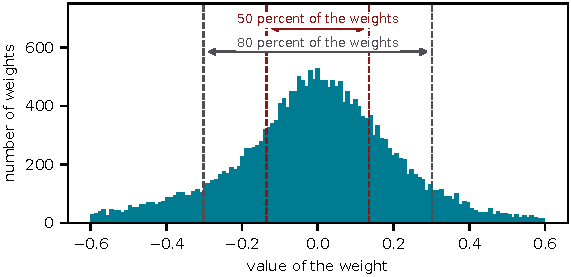
\includegraphics[width=0.74\textwidth]{images/day06/weight_histogram.pdf}
  \par\endgroup
  \small
  \begin{itemize}
    \item A trained network has many weights near 0. Such a weight changes
          the output of its layer very little.
    \item Pruning sets these weights to exactly 0. The \textbf{sparsity} is
          the part of the weights that are 0.
  \end{itemize}
  \source{The weights of the example model of this part: a CNN for
    Fashion-MNIST with 23\,824 weights in its kernels.}
\end{frame}

\begin{frame}{The example model of this part}
  \small
  \renewcommand{\arraystretch}{1.2}
  \begin{tabular}{@{}L{0.42\textwidth}L{0.24\textwidth}r@{}}
    \toprule
    \textbf{Layer} & \textbf{Output} & \textbf{Weights} \\
    \midrule
    Input: image $28 \times 28$, 1 channel & $28 \times 28 \times 1$
        & none \\
    Convolution $3 \times 3$, 16 filters, then pooling
        & $14 \times 14 \times 16$ & 144 \\
    Convolution $3 \times 3$, 32 filters, then pooling
        & $7 \times 7 \times 32$ & 4608 \\
    Convolution $3 \times 3$, 64 filters, then global pooling
        & 64 & 18\,432 \\
    Fully connected, softmax & 10 & 640 \\
    \bottomrule
  \end{tabular}
  \vskip 0.5em
  \begin{itemize}
    \item 23\,946 parameters with the biases. Accuracy on the test set:
          89.1 percent.
    \item 1.92 million MACs. Peak of the activations: 15\,680 values.
    \item LiteRT file in \code{float32}: 99\,320 bytes. Latency on a laptop
          CPU with one thread: 66 microseconds.
  \end{itemize}
  \source{An experiment of this course with Fashion-MNIST (10 classes of
    clothes, images of $28 \times 28$). The lab of today uses the same
    model.}
\end{frame}

% ------------------------------------------------------------------ criteria
\begin{frame}{Magnitude pruning}
  \begin{columns}[c]
    \begin{column}{0.48\textwidth}
      \[
        \hat{W} = M \odot W
      \]
      \[
        M_{ij} = \begin{cases} 1 & \text{if } |W_{ij}| > \delta \\
                               0 & \text{in all other cases}
                 \end{cases}
      \]
    \end{column}
    \begin{column}{0.50\textwidth}
      \small
      \begin{tabular}{@{}rL{0.62\textwidth}@{}}
        $W$ & The weights of a layer \\
        $M$ & The mask: 1 for a weight that stays, 0 for a weight that
              goes \\
        $\odot$ & The product of each weight with its mask value \\
        $\delta$ & The threshold \\
      \end{tabular}
    \end{column}
  \end{columns}
  \vskip 0.5em
  \begin{itemize}
    \item The criterion is the magnitude: the absolute value of the weight.
    \item You select the sparsity, for example 80 percent. The threshold is
          then the magnitude that 80 percent of the weights are below.
    \item For the example model: $\delta = 0.135$ for 50 percent, and
          $\delta = 0.301$ for 80 percent.
  \end{itemize}
  \source{Formula: \emph{Machine Learning Systems}, Volume I, chapter 10.
    Threshold values: the example model.}
\end{frame}

\begin{frame}{Other criteria}
  \small
  \renewcommand{\arraystretch}{1.2}
  \begin{tabular}{@{}L{0.16\textwidth}L{0.42\textwidth}L{0.32\textwidth}@{}}
    \toprule
    \textbf{Criterion} & \textbf{The score of a weight or a filter}
    & \textbf{Cost} \\
    \midrule
    Magnitude  & The absolute value, or the sum of the absolute values of
                 a filter & None: the weights are enough \\
    Gradient   & The weight times its gradient: the change of the loss
                 when the weight goes & One pass over some data \\
    Activation & The mean output of a filter on real data: a filter that
                 is almost always 0 goes & One pass over some data \\
    Random     & No score & None. It is the baseline for a comparison. \\
    \bottomrule
  \end{tabular}
  \vskip 0.6em
  \begin{itemize}
    \item The problem ``find the best set of weights to remove'' has no
          fast exact solution. All criteria are estimates.
    \item Magnitude is the standard: it is simple, and it works well with
          fine-tuning.
  \end{itemize}
\end{frame}

\begin{frame}{Local and global thresholds}
  \small
  \renewcommand{\arraystretch}{1.25}
  \begin{tabular}{@{}L{0.30\textwidth}rrr@{}}
    \toprule
    \textbf{Layer} & \textbf{Weights} & \textbf{Local, 80 percent}
    & \textbf{Global, 80 percent} \\
    \midrule
    Convolution 1   & 144     & 80 & 51 \\
    Convolution 2   & 4608    & 80 & 71 \\
    Convolution 3   & 18\,432 & 80 & 83 \\
    Fully connected & 640     & 80 & 63 \\
    \bottomrule
  \end{tabular}
  \vskip 0.5em
  \begin{itemize}
    \item \textbf{Local:} each layer has its own threshold. Each layer loses
          the same part of its weights.
    \item \textbf{Global:} one threshold for all layers. The table gives the
          sparsity in percent that each layer gets.
    \item With the global threshold, the first layer keeps half of its
          weights. It is small, and each of its weights is used at all
          positions of the image.
    \item The large layer loses most. This is the layer with the most
          redundancy.
  \end{itemize}
  \source{Sparsity of each layer: the example model with a global sparsity
    of 80 percent.}
\end{frame}

% --------------------------------------------------------------- fine-tuning
\begin{frame}{Fine-tuning brings the accuracy back}
  \begin{columns}[c]
    \begin{column}{0.50\textwidth}
      \centering
      \begin{tikzpicture}[font=\scriptsize, x=0.078cm, y=0.038cm]
        \draw[->, coolgray] (40,0) -- (100,0);
        \node[coolgray] at (70,-18) {sparsity in percent};
        \draw[->, coolgray] (40,0) -- (40,104);
        \node[anchor=west, coolgray] at (41,104) {accuracy};
        \foreach \x in {50,70,80,90} {
          \draw[coolgray] (\x,0) -- (\x,-2) node[below] {\x};
        }
        \draw[coolgray] (95,0) -- (95,-2);
        \foreach \y in {50,89} {
          \draw[coolgray] (40,\y) -- (39,\y) node[left] {\y};
        }
        \draw[coolgray!50, dashed] (40,89.1) -- (98,89.1);
        \draw[coolgray, line width=0.9pt] plot coordinates
          {(50,79.9) (70,50.9) (80,23.4) (90,10.0) (95,10.0)};
        \draw[cardinalred, line width=1.1pt] plot coordinates
          {(50,90.0) (70,88.8) (80,85.7) (90,76.4) (95,51.0)};
        \foreach \x/\y in {50/90.0, 70/88.8, 80/85.7, 90/76.4, 95/51.0} {
          \fill[cardinalred] (\x,\y) circle (1.6pt);
        }
        \node[cardinalred, anchor=west] at (44,97) {after fine-tuning};
        \node[coolgray, anchor=west] at (43,40) {before};
      \end{tikzpicture}
    \end{column}
    \begin{column}{0.46\textwidth}
      \small
      \begin{itemize}
        \item After the pruning, the accuracy falls: to 23.4 percent at a
              sparsity of 80 percent.
        \item \textbf{Fine-tuning:} train again for some epochs, with a
              small learning rate. The mask stays: a weight that is 0
              stays 0.
        \item The other weights take the work of the removed weights.
        \item At 50 percent, the pruned model is better than the baseline:
              90.0 against 89.1.
      \end{itemize}
    \end{column}
  \end{columns}
  \vskip 0.2em
  \source{The example model, global magnitude pruning, 2 epochs of
    fine-tuning. Accuracy in percent on the test set.}
\end{frame}

\begin{frame}{Schedules: one-shot and iterative}
  \begingroup\centering
  \begin{tikzpicture}[font=\footnotesize, >={Stealth[length=5pt]},
      b/.style={draw=coolgray, rounded corners=3pt, fill=boxgray,
                minimum width=1.5cm, minimum height=0.75cm, align=center},
      p/.style={b, draw=cardinalred},
      lab/.style={font=\scriptsize, text=coolgray}]
    \node[lab, anchor=east] at (-1.0,0) {One-shot};
    \node[b] (a) at (0,0) {Train};
    \node[p] (b) at (2.2,0) {Prune 90};
    \node[b] (c) at (4.4,0) {Fine-tune};
    \draw[->] (a) -- (b); \draw[->] (b) -- (c);
    \node[lab, anchor=east] at (-1.0,-1.1) {Iterative};
    \node[b] (d) at (0,-1.1) {Train};
    \node[p] (e) at (2.2,-1.1) {Prune 50};
    \node[b] (f) at (4.4,-1.1) {Fine-tune};
    \node[p] (g) at (6.6,-1.1) {Prune 75};
    \node[lab] (h) at (8.2,-1.1) {\dots\ 90};
    \draw[->] (d) -- (e); \draw[->] (e) -- (f); \draw[->] (f) -- (g);
    \draw[->] (g) -- (h);
  \end{tikzpicture}\par\endgroup
  \vskip 0.4em
  \small
  \begin{itemize}
    \item \textbf{One-shot:} remove all weights in one step. It is fast. At
          a high sparsity, the model can lose too much to recover.
    \item \textbf{Iterative:} remove a part, fine-tune, and repeat. The
          model adapts in small steps. It costs one fine-tuning for each
          step.
    \item An example of the book with channel pruning of 27 percent: the
          iterative schedule loses 0.4 points, and the one-shot schedule
          loses 5 points.
    \item The example model of this part, to a sparsity of 90 percent with
          3 epochs for each schedule: 78.4 percent (one-shot) and 77.3
          percent (iterative). No gain: the result depends on the model.
  \end{itemize}
  \source{Example of the book: \emph{Machine Learning Systems}, Volume I,
    chapter 10.}
\end{frame}

\begin{frame}{The lottery ticket hypothesis}
  \begin{columns}[T]
    \begin{column}{0.50\textwidth}
      \begin{block}{The hypothesis}
        A large network holds a small subnetwork that reaches almost the
        same accuracy when you train it alone, from its first random
        weights. This subnetwork is the ``winning ticket''.
      \end{block}
    \end{column}
    \begin{column}{0.46\textwidth}
      \begin{block}{How to find it}
        \begin{enumerate}
          \item Train the network.
          \item Prune the small weights.
          \item Set the other weights back to their first values.
          \item Repeat.
        \end{enumerate}
      \end{block}
    \end{column}
  \end{columns}
  \vskip 0.5em
  \begin{itemize}
    \item The result explains why pruning works: most weights help the
          training, and the trained function needs only some of them.
    \item It is not a method to save training time: you find the ticket
          only after you trained the large network.
    \item For this course, the practical result is: start large, then
          prune. Do not start with a network that is too small.
  \end{itemize}
  \source{Frankle and Carbin, ``The Lottery Ticket Hypothesis'', 2019.}
\end{frame}

% ------------------------------------------------------------ what you gain
\begin{frame}{Granularity: what you remove}
  \begingroup\centering
  \begin{tikzpicture}[font=\scriptsize, x=0.33cm, y=0.33cm]
    % Left: unstructured. A matrix of 8 x 8 with single zeros.
    \foreach \i in {0,...,7} { \foreach \j in {0,...,7} {
      \draw[coolgray!60, fill=darkcyan!45] (\i,\j) rectangle (\i+1,\j+1);
    } }
    \foreach \i/\j in {0/1, 0/4, 0/6, 1/0, 1/2, 1/3, 1/7, 2/1, 2/5, 2/6,
                       3/0, 3/2, 3/4, 3/7, 4/1, 4/3, 4/5, 4/6, 5/0, 5/2,
                       5/4, 5/7, 6/1, 6/3, 6/5, 6/6, 7/0, 7/2, 7/4, 7/7,
                       0/2, 2/3} {
      \draw[coolgray!60, fill=white] (\i,\j) rectangle (\i+1,\j+1);
    }
    \node[below] at (4,-0.2) {Unstructured: single weights};
    % Right: structured. Complete columns removed.
    \begin{scope}[shift={(13,0)}]
      \foreach \i in {0,...,7} { \foreach \j in {0,...,7} {
        \draw[coolgray!60, fill=darkcyan!45] (\i,\j) rectangle (\i+1,\j+1);
      } }
      \foreach \i in {1,3,4,6} { \foreach \j in {0,...,7} {
        \draw[coolgray!60, fill=white] (\i,\j) rectangle (\i+1,\j+1);
      } }
      \node[below] at (4,-0.2) {Structured: complete filters};
    \end{scope}
    \node[coolgray] at (10.5,4) {white = 0};
  \end{tikzpicture}\par\endgroup
  \vskip 0.3em
  \small
  \begin{itemize}
    \item \textbf{Unstructured:} each weight is a candidate. The tensor
          keeps its shape and gets zeros at irregular positions.
    \item \textbf{Structured:} a complete unit is a candidate: a neuron, a
          filter with its channel, or a layer. The tensor becomes smaller.
    \item The two figures have the same sparsity: 50 percent. The device
          sees two very different models.
  \end{itemize}
  \keypoint{Unstructured pruning has more freedom, so it keeps more
    accuracy. Structured pruning gives a model that normal hardware runs
    faster.}
\end{frame}

\begin{frame}{A sparse model in the flash}
  \small
  \renewcommand{\arraystretch}{1.25}
  \begin{tabular}{@{}L{0.18\textwidth}rrrr@{}}
    \toprule
    \textbf{Sparsity} & \textbf{Weights not 0} & \textbf{LiteRT file}
    & \textbf{After gzip} & \textbf{Sparse format} \\
    \midrule
    None & 23\,824 & 99\,320 & 90\,877 & not useful \\
    50 percent & 11\,912 & 99\,320 & 54\,423 & 71\,472 \\
    80 percent & 4764    & 99\,320 & 27\,498 & 28\,584 \\
    90 percent & 2383    & 99\,320 & 17\,796 & 14\,298 \\
    \bottomrule
  \end{tabular}
  \vskip 0.5em
  \begin{itemize}
    \item All sizes are in bytes. The file does not change: a zero in
          \code{float32} needs 4 bytes, as each other value.
    \item A compression tool makes the file smaller. But the runtime of a
          microcontroller reads the model in place from the flash. It
          cannot read a compressed file.
    \item A sparse format stores each value with its position. The column
          gives 4 bytes for a value and 2 bytes for an index. The weights
          alone need 95\,296 bytes in the dense format.
  \end{itemize}
  \source{File sizes: the example model. Sparse format: a calculation with
    6 bytes for each weight that is not 0.}
\end{frame}

\begin{frame}{Why zeros do not make a processor faster}
  \begin{columns}[T]
    \begin{column}{0.48\textwidth}
      \begin{block}{A dense kernel}
        \begin{itemize}
          \item A loop over all weights, in order.
          \item The processor multiplies 4, 8, or 16 values in one
                instruction.
          \item A multiplication by 0 costs the same time as each other
                multiplication.
        \end{itemize}
      \end{block}
    \end{column}
    \begin{column}{0.48\textwidth}
      \begin{block}{A sparse kernel}
        \begin{itemize}
          \item It reads the position of each value first.
          \item It jumps in the memory. The cache and the wide
                instructions help less.
          \item It is faster only at a high sparsity, often above 80 to
                90 percent.
        \end{itemize}
      \end{block}
    \end{column}
  \end{columns}
  \vskip 0.5em
  \begin{itemize}
    \item The kernels of LiteRT and of TensorFlow Lite Micro are dense
          kernels. Some runtimes have sparse kernels for some layer types.
  \end{itemize}
  \keypoint{Sparsity is a property of the model. Speed is a property of the
    model, the runtime, and the hardware together.}
  \source{Break-even sparsity: \emph{Machine Learning Systems}, Volume I,
    chapter 10.}
\end{frame}

\begin{frame}{Measured: sparsity and latency}
  \begingroup\centering
  \begin{tikzpicture}[font=\scriptsize, x=1.05cm, y=0.034cm]
    \draw[->, coolgray] (0,0) -- (9.3,0);
    \draw[->, coolgray] (0,0) -- (0,100);
    \node[anchor=west, coolgray] at (0.1,98) {latency in microseconds};
    \foreach \y in {25,50,75} {
      \draw[coolgray] (0,\y) -- (-0.08,\y) node[left] {\y};
      \draw[coolgray!40, dotted] (0,\y) -- (9.1,\y);
    }
    \foreach \k/\v/\l in {1/66/dense, 2/82/50, 3/73/70, 4/73/80, 5/66/90} {
      \fill[darkcyan!55] (\k-0.33,0) rectangle (\k+0.33,\v);
      \node[above] at (\k,\v) {\v};
      \node[below] at (\k,0) {\l};
    }
    \foreach \k/\v/\l in {6.6/54/0.75, 7.6/32/0.5, 8.6/21/0.25} {
      \fill[cardinalred!60] (\k-0.33,0) rectangle (\k+0.33,\v);
      \node[above] at (\k,\v) {\v};
      \node[below] at (\k,0) {\l};
    }
    \node[darkcyan!70!black] at (3.5,-18) {unstructured: sparsity in
      percent};
    \node[cardinalred] at (7.6,-18) {structured: part of the filters};
  \end{tikzpicture}\par\endgroup
  \vskip 0.3em
  \small
  \begin{itemize}
    \item Unstructured: the latency stays between 66 and 82 microseconds.
          The differences are noise of the measurement. The zeros give no
          gain.
    \item Structured: with half of the filters in each layer, the latency
          falls from 66 to 32 microseconds.
  \end{itemize}
  \source{The example model with LiteRT on a laptop CPU, one thread, median
    of 5 runs. The values say nothing about a board.}
\end{frame}

% ---------------------------------------------------------------- structured
\begin{frame}{Structured pruning: remove a filter}
  \begingroup\centering
  \begin{tikzpicture}[font=\scriptsize, >={Stealth[length=4pt]}]
    % Layer k: 4 filters. Layer k+1: kernels with 4 input channels.
    \foreach \i/\c in {0/boxgray, 1/cardinalred!35, 2/boxgray, 3/boxgray} {
      \draw[coolgray, fill=\c] (0,-0.55*\i) rectangle (1.6,-0.55*\i+0.4);
    }
    \node[above] at (0.8,0.45) {filters of layer $k$};
    \foreach \i/\c in {0/boxgray, 1/cardinalred!35, 2/boxgray, 3/boxgray} {
      \draw[coolgray, fill=\c] (3.2,-0.55*\i) rectangle (4.0,-0.55*\i+0.4);
      \draw[->, coolgray] (1.65,-0.55*\i+0.2) -- (3.15,-0.55*\i+0.2);
    }
    \node[above] at (3.6,0.45) {its output channels};
    \foreach \f in {0,1,2} {
      \foreach \i/\c in {0/boxgray, 1/cardinalred!35, 2/boxgray, 3/boxgray} {
        \draw[coolgray, fill=\c] (5.6+1.2*\f,-0.55*\i)
          rectangle (6.5+1.2*\f,-0.55*\i+0.4);
      }
    }
    \node[above] at (7.25,0.45) {filters of layer $k+1$};
    \draw[->, coolgray] (4.05,-0.6) -- (5.55,-0.6);
  \end{tikzpicture}\par\endgroup
  \vskip 0.4em
  \small
  \begin{itemize}
    \item A filter of layer $k$ makes one output channel. Without the
          filter, the channel does not exist.
    \item So each filter of layer $k+1$ loses its weights for this channel.
    \item One removed filter makes two layers smaller, and it removes one
          feature map from the RAM.
    \item A usual criterion: the sum of the absolute values of the weights
          of the filter. Remove the filters with the smallest sum.
  \end{itemize}
  \keypoint{The result is a normal, smaller, dense model. Each runtime runs
    it with no change.}
\end{frame}

\begin{frame}{Structured pruning of the example model}
  \small
  \renewcommand{\arraystretch}{1.25}
  \setlength{\tabcolsep}{4pt}
  \begin{tabular}{@{}L{0.14\textwidth}rrrrrr@{}}
    \toprule
    \textbf{Filters} & \textbf{Parameters} & \textbf{MACs}
    & \textbf{Accuracy} & \textbf{File} & \textbf{Latency}
    & \textbf{Peak} \\
    \midrule
    16, 32, 64 & 23\,946 & 1\,919\,872 & 89.1 & 99\,320 & 66 & 15\,680 \\
    12, 24, 48 & 13\,642 & 1\,101\,216 & 88.8 & 58\,104 & 54 & 11\,760 \\
    8, 16, 32  & 6218    & 508\,352    & 85.6 & 28\,408 & 32 & 7840 \\
    4, 8, 16   & 1674    & 141\,280    & 76.2 & 10\,232 & 21 & 3920 \\
    \bottomrule
  \end{tabular}
  \vskip 0.5em
  \begin{itemize}
    \item Accuracy in percent after 2 epochs of fine-tuning. File in bytes,
          latency in microseconds, peak of the activations in values.
    \item With three quarters of the filters, the model loses 0.3 points
          and 41 percent of its file.
    \item With half of the filters, the MACs fall by a factor of 3.8. The
          latency falls by a factor of 2.1 only: the time has a part that
          does not depend on the MACs.
    \item The peak falls with the number of filters. Unstructured pruning
          does not change the peak.
  \end{itemize}
  \source{The example model with LiteRT on a laptop CPU, one thread.}
\end{frame}

\begin{frame}{The same accuracy, two different models}
  \small
  \renewcommand{\arraystretch}{1.3}
  \begin{tabular}{@{}L{0.36\textwidth}rr@{}}
    \toprule
    & \textbf{Unstructured, 80 percent} & \textbf{Structured, half} \\
    \midrule
    Accuracy in percent      & 85.7     & 85.6 \\
    Weights not 0            & 4764     & 6152 \\
    File in bytes            & 99\,320  & 28\,408 \\
    Latency in microseconds  & 73       & 32 \\
    Peak of the activations  & 15\,680  & 7840 \\
    \bottomrule
  \end{tabular}
  \vskip 0.6em
  \begin{itemize}
    \item The unstructured model keeps fewer weights for the same accuracy.
          It has more freedom to select them.
    \item The structured model has half of the filters in each layer. It is
          better in each number that the device sees: flash, time, and
          RAM.
  \end{itemize}
  \keypoint{With dense kernels, only structured pruning pays. Unstructured
    pruning pays when the download of the file is the limit.}
  \source{The example model. Structured: 6152 weights and 66 biases.}
\end{frame}

\begin{frame}{Who gains from which pruning}
  \small
  \renewcommand{\arraystretch}{1.3}
  \begin{tabular}{@{}L{0.36\textwidth}L{0.26\textwidth}L{0.28\textwidth}@{}}
    \toprule
    \textbf{Target} & \textbf{Unstructured} & \textbf{Structured} \\
    \midrule
    Microcontroller with TensorFlow Lite Micro
        & No gain & Flash, RAM, and time \\
    Raspberry Pi with LiteRT
        & No gain in time & Flash, RAM, and time \\
    A runtime with sparse kernels
        & Time, at a high sparsity & Time \\
    The download of a model over a slow network
        & A smaller compressed file & A smaller file \\
    \bottomrule
  \end{tabular}
  \vskip 0.6em
  \begin{itemize}
    \item The table is the rule of this course for its two boards.
    \item Many papers report the sparsity or the number of parameters
          only. These numbers do not tell you the gain on your device.
  \end{itemize}
  \keypoint{Before you prune, ask: which kernels does my runtime have? Then
    measure the pruned model on the device.}
\end{frame}

\begin{frame}{Pruning in practice}
  \begingroup\centering
  \begin{tikzpicture}[font=\footnotesize, >={Stealth[length=5pt]},
      b/.style={draw=coolgray, rounded corners=3pt, fill=boxgray,
                minimum width=1.75cm, minimum height=1.0cm, align=center}]
    \node[b] (a) at (0,0)    {Trained\\model};
    \node[b, draw=cardinalred] (b) at (2.15,0) {Prune};
    \node[b] (c) at (4.3,0)  {Fine-tune};
    \node[b] (d) at (6.45,0) {Export};
    \node[b, draw=darkcyan] (e) at (8.6,0)  {Measure on\\the device};
    \foreach \a/\b in {a/b, b/c, c/d, d/e} { \draw[->] (\a) -- (\b); }
    \draw[->, coolgray] (c.south) -- ++(0,-0.5) -| (b.south);
  \end{tikzpicture}\par\endgroup
  \vskip 0.5em
  \begin{itemize}
    \item \textbf{Prune and fine-tune} a trained model in some steps. After
          each step, write the accuracy.
    \item \textbf{Export.} For structured pruning, build the smaller model
          and copy the weights that stay. A mask alone saves nothing: the
          tensor still has its full size.
    \item \textbf{Measure} the file, the latency, and the RAM of the
          exported model on the device.
    \item \textbf{Then quantize.} Pruning and quantization multiply: fewer
          values, and fewer bits for each value.
  \end{itemize}
  \keypoint{The pruned model of the training tool is not the model of the
    device. Only the exported file counts.}
\end{frame}

\begin{frame}{The limits of pruning}
  \begin{columns}[T]
    \begin{column}{0.48\textwidth}
      \begin{block}{What pruning cannot do}
        \begin{itemize}
          \item It keeps the architecture: the same layer types and the
                same connections.
          \item It cannot change the input size or the first feature map.
          \item A model that was small from the start has little to
                remove.
        \end{itemize}
      \end{block}
    \end{column}
    \begin{column}{0.48\textwidth}
      \begin{block}{The curve has a knee}
        \begin{itemize}
          \item To a sparsity of 70 percent, the example model loses 0.3
                points.
          \item From 80 to 90 percent, it loses 9 points.
          \item Stop before the knee.
        \end{itemize}
      \end{block}
    \end{column}
  \end{columns}
  \vskip 0.5em
  \begin{itemize}
    \item When the target needs a different architecture, pruning is the
          wrong tool. Part 2 gives a method that trains a new, smaller
          model with the help of the large model.
  \end{itemize}
  \source{Accuracy values: the example model with unstructured pruning and
    2 epochs of fine-tuning.}
\end{frame}

% -------------------------------------------------------------------- exercise
\exerciseframe{predict the latency of a sparse model}{%
  \small
  A model runs with LiteRT on the processor of a Raspberry Pi. It uses the
  normal, dense kernels.
  \vskip 0.2em
  {\footnotesize
  \renewcommand{\arraystretch}{1.1}
  \begin{tabular}{@{}L{0.50\textwidth}r@{}}
    \toprule
    Parameters & 2.0 million \\
    MACs for one inference & 300 million \\
    File in \code{float32} & 7.6 MB \\
    Latency & 60 ms \\
    \bottomrule
  \end{tabular}}
  \vskip 0.2em
  A colleague prunes the model with unstructured magnitude pruning to a
  sparsity of 80 percent. The accuracy stays almost equal. The colleague
  says: ``The model is now 5 times as fast and 5 times as small.''
  \begin{enumerate}
    \item Predict the latency of the pruned model. Give the reason.
    \item Predict the size of the model file. How can the file become
          smaller?
    \item The target is 30 ms. Propose a pruning method that can reach it.
          Which part of the channels do you remove, if the MACs of a
          convolution grow with the square of the number of channels?
    \item Which of the two methods makes the peak RAM smaller?
  \end{enumerate}
}

\answerframe{predict the latency of a sparse model}{%
  \small
  \begin{enumerate}
    \item About 60 ms: no change. The dense kernels multiply each weight,
          also a weight that is 0. The model still does 300 million MACs.
          A sparse kernel gives a gain only at a high sparsity, and only
          if the runtime has one for the layers of the model.
    \item 7.6 MB: no change. Each zero needs 4 bytes. A sparse format with
          4 bytes for a value and 2 bytes for an index needs
          $400\,000 \times 6$ bytes: 2.3 MB. A compression tool also helps for
          the download, but not for the memory at run time.
    \item Structured pruning: remove complete filters. For half of the
          time, you need about half of the MACs. With $c^2 = 0.5$, the
          part of the channels that stays is $c = 0.71$. Remove about 30
          percent of the channels of each layer. The example of this part
          shows that the time falls less than the MACs, so plan for 35 to
          40 percent, and measure.
    \item Structured pruning. Fewer channels give smaller feature maps.
          Unstructured pruning keeps the shape of each tensor, so the peak
          RAM does not change.
  \end{enumerate}
  \vskip 0.1em
  After each of the two methods, measure the accuracy again.
}

% Part 2 of Day 6: Knowledge distillation and low-rank methods.
%
% Topics of the syllabus: soft targets and temperature; feature distillation;
% low-rank factorization. Exercise: calculate soft targets at two
% temperatures.

\theorypart{Knowledge distillation and low-rank methods}%
  {calculate soft targets at two temperatures}

% Part 3 of Day 6: Efficient design and technique selection.
%
% Topics of the syllabus: MobileNet, EfficientNet, and MCUNet; hardware-aware
% neural architecture search; order of techniques: prune, distill, quantize.
% Exercise: select techniques for three cases (flash limit, RAM limit, latency
% limit).

\theorypart{Efficient design and technique selection}%
  {select techniques for three cases}

% Recap of the day. Three to five points, then the one point to keep.
\begin{frame}{Recap}
  \begin{itemize}
    \item Unstructured pruning makes the model file smaller. Only structured
          pruning makes a normal runtime faster.
    \item Distillation trains a small student with the soft outputs of a large
          teacher. The temperature controls how much the small probabilities
          count.
    \item An efficient design decreases the operations and the activations
          before the training starts.
    \item The constraint selects the technique: flash, RAM, or latency. The
          usual order is prune, distill, quantize.
  \end{itemize}
  \vskip 0.5em
  \keypoint{Measure each technique on the target device. A smaller number of
            parameters is not a smaller latency, and it is not a smaller peak
            RAM.}
\end{frame}

% Further reading. The list comes from the "Sources" part of Day 6 in the
% syllabus.
\begin{frame}{Further reading}
  \footnotesize
  \begin{block}{Book chapters}
    \begin{itemize}
      \item \emph{Machine Learning Systems} (mlsysbook.ai), Volume I: chapter
            10 ``Model Compression'', sections ``Structural Optimization'',
            ``Architectural Efficiency'', and ``Technique Selection''.
    \end{itemize}
  \end{block}
  \begin{block}{Papers}
    \begin{itemize}
      \item ``Learning both Weights and Connections for Efficient Neural
            Networks'', Han et al., 2015.
      \item ``The Lottery Ticket Hypothesis: Finding Sparse, Trainable Neural
            Networks'', Frankle and Carbin, 2019.
      \item ``Distilling the Knowledge in a Neural Network'', Hinton et al.,
            2015.
      \item ``EfficientNet: Rethinking Model Scaling for Convolutional Neural
            Networks'', Tan and Le, 2019.
      \item ``MCUNet: Tiny Deep Learning on IoT Devices'', Lin et al., 2020.
    \end{itemize}
  \end{block}
  \begin{block}{Course}
    \begin{itemize}
      \item MIT 6.5940 ``TinyML and Efficient Deep Learning Computing'', for
            more depth: \url{https://efficientml.ai}
    \end{itemize}
  \end{block}
\end{frame}

% Credits frame. Section 10 of the syllabus gives this text.
% Each deck ends with this frame:
%   % Credits frame. Section 10 of the syllabus gives this text.
% Each deck ends with this frame:
%   % Credits frame. Section 10 of the syllabus gives this text.
% Each deck ends with this frame:
%   \input{sections/credits}
%
% The list \coursecredits selects the sources. preamble/course.tex gives the
% default list and one command for each source. The main file of a deck
% changes the list before it inputs this file, so that the frame names only
% the sources that the deck uses:
%   \renewcommand{\coursecredits}{\creditmlsys\creditxiao}
\begin{frame}[allowframebreaks]{Credits}
  \vskip 0.6em
  \begin{itemize}\footnotesize\itemsep 0.4em
    \coursecredits
  \end{itemize}
  \vskip 0.8em
\end{frame}

%
% The list \coursecredits selects the sources. preamble/course.tex gives the
% default list and one command for each source. The main file of a deck
% changes the list before it inputs this file, so that the frame names only
% the sources that the deck uses:
%   \renewcommand{\coursecredits}{\creditmlsys\creditxiao}
\begin{frame}[allowframebreaks]{Credits}
  \vskip 0.6em
  \begin{itemize}\footnotesize\itemsep 0.4em
    \coursecredits
  \end{itemize}
  \vskip 0.8em
\end{frame}

%
% The list \coursecredits selects the sources. preamble/course.tex gives the
% default list and one command for each source. The main file of a deck
% changes the list before it inputs this file, so that the frame names only
% the sources that the deck uses:
%   \renewcommand{\coursecredits}{\creditmlsys\creditxiao}
\begin{frame}[allowframebreaks]{Credits}
  \vskip 0.6em
  \begin{itemize}\footnotesize\itemsep 0.4em
    \coursecredits
  \end{itemize}
  \vskip 0.8em
\end{frame}


\end{document}
